%=======================================================================
%  CENG318 Human-Computer Interaction - Spring 2026
%  FINAL PROJECT REPORT  -  Project: BarberNearMe
%  SINGLE-COLUMN FALLBACK VERSION - matches the original instructor
%  template's article-class / chicago-style format, in case the
%  IEEE-conference instruction turns out not to apply this semester.
%  Content is identical to the IEEE version; only the document class,
%  title block, and bibliography style differ.
%
%  Build:  pdflatex  ->  bibtex  ->  pdflatex  ->  pdflatex
%=======================================================================
\documentclass[14pt]{article}
\usepackage{graphics}
\usepackage{epsfig}
\usepackage{times}
\usepackage{amsmath}
\usepackage{subcaption}
\usepackage{multirow}
\usepackage{gensymb}
\usepackage{array}
\usepackage{float}
\usepackage{indentfirst}
\usepackage[table]{xcolor}
\newcolumntype{P}[1]{>{\centering\arraybackslash}p{#1}}
\usepackage{booktabs, makecell}
\usepackage{diagbox}
\usepackage{float}
\floatstyle{plaintop}
\restylefloat{table}
\usepackage{natbib}
\usepackage{url}
\usepackage[hidelinks]{hyperref}

\topmargin      0.0in
\headheight     0.0in
\headsep        0.0in
\oddsidemargin  0.0in
\evensidemargin 0.0in
\textheight     9.0in
\textwidth      6.5in

% Status colors for the project-plan (Gantt) table.
\definecolor{doneG}{RGB}{183,228,199}   % green  = finished
\definecolor{progB}{RGB}{190,212,245}   % blue   = in progress
\definecolor{planY}{RGB}{251,229,160}   % yellow = planned / future
\newcommand{\cD}{\cellcolor{doneG}}
\newcommand{\cP}{\cellcolor{progB}}
\newcommand{\cY}{\cellcolor{planY}}

\title{{\bf CENG318 Human Computer Interaction\\ Spring 2026} \\
	{Project Title: BarberNearMe}\\
	Group 19 Final Report}

\date{\today}

\begin{document}

\pagestyle{plain}
\pagenumbering{roman}
\maketitle

\begin{figure}[H]
	\centering
	
\includegraphics[width=1.3in]{iyte_logo}
\end{figure}

\textbf{ Group Members}
\begin{itemize}
	\item Vedat Demir 280201047
	\item Osman Said Tekin 270201010
	\item Burak Rahmanoğlu 290201030
	\item Batuhan Mutlu 300201094
	\item Enes Ergün Hoşgör 300201053
\end{itemize}

\cleardoublepage
\pagenumbering{arabic}

\abstract{
BarberNearMe is a cross-platform mobile application that connects
customers with nearby barbershops and digitises an appointment lifecycle
still dominated by walk-ins and phone calls. This report documents the
move from proposal to a working prototype, organised around the three
pillars introduced earlier: Discovery, Interaction, and Reliability. For
Discovery, the app combines device GPS, an interactive map, and
client-side Haversine distance computation to rank shops by proximity,
rating, price, and open-now status. For Interaction, customers browse
shop details, book conflict-free time slots, manage and cancel
appointments, exchange real-time messages with shops, and rate completed
visits; barbers register a shop through a multi-step wizard and manage
appointments from a dashboard. For Reliability, reviews are gated so that
only the customer of a \emph{completed} appointment may post exactly one
review per visit, structurally enforcing the verified-only rating goal.
During development the stack changed substantially: instead of an
Android/Kotlin client with a .NET~8 REST API over PostgreSQL, the team
built an Expo / React~Native (TypeScript) client backed by Firebase
Authentication and Cloud Firestore, accessed through a dedicated service
layer. The payment step uses a mock deposit flow secured by Luhn
check-digit validation, verified against a 100-card test set (50 valid,
50 invalid) with 100\% classification accuracy; one proposal item
remains open: the AI head-shape styling module is future work.
Formal usability evaluation (System Usability Scale) and performance
benchmarking were planned but not yet executed; their methodology is
specified here and their results are explicitly marked as pending. The
outcome is a functional, end-to-end booking prototype with a clearly
scoped path to completion.
}

\cleardoublepage

\section{Introduction}
%-----------------------------------------------------------------------
Personal-care services such as barbershops still rely heavily on manual
booking and word-of-mouth reputation. \emph{BarberNearMe} targets this
gap with a single mobile application where customers discover well-rated
local barbers, book a slot, communicate with the shop, and leave
trustworthy feedback. This document is a progress report: rather than
restating intentions, it records what was built, what diverged from the
proposal, and what remains.

The project addresses three concrete problems that motivated the design:

\begin{itemize}
  \item \textbf{Service uncertainty and wait times.} Customers cannot
        easily compare nearby shops or see availability before showing
        up. BarberNearMe answers this with map- and list-based discovery,
        proximity ranking, an open-now filter, and a calendar that
        disables already-booked slots to prevent double-booking.
  \item \textbf{The trust deficit in reviews.} Most platforms let anyone
        post a rating. BarberNearMe ties every review to a specific
        completed appointment owned by the reviewer and permits exactly
        one review per appointment, so feedback comes only from people
        who actually received the service.
  \item \textbf{The styling mismatch.} A chosen hairstyle may not suit a
        customer's features. This is the most forward-looking problem:
        the architecture leaves room for an image-based head-shape
        analysis module, which is documented here as future work rather
        than a delivered feature.
\end{itemize}

The remainder of the report reviews related work and positions the
novelty of the approach (Section~\ref{sec:lit}), describes what was
actually implemented across the six planned stages
(Section~\ref{sec:method}), states the evaluation plan and the current
evidence (Section~\ref{sec:exp}), and concludes with an honest account
of remaining work (Section~\ref{sec:concl}).

%-----------------------------------------------------------------------
\section{Literature Review}
\label{sec:lit}
%-----------------------------------------------------------------------
Commercial scheduling platforms such as Booker and StyleSeat focus mainly
on administrative booking and calendar management. They are effective for
shop owners but offer limited support for the two problems most relevant
here: the authenticity of reviews and the match between a hairstyle and a
customer's physical features. In particular, these platforms generally do
not verify that a reviewer actually received the service, which makes
ratings vulnerable to bias, and they provide no visual guidance for style
compatibility.

From a human-computer interaction standpoint, the design of BarberNearMe
follows established usability principles---consistency, user control,
recognition over recall, and clear feedback---as articulated by
\citet{shneiderman2016designing}. These
principles are reflected concretely in the prototype: a persistent
bottom-tab structure, status badges on appointments, disabled time slots
that communicate availability at a glance, and confirmation dialogs
before destructive actions such as cancellation.

The novelty of BarberNearMe relative to existing tools is the combination
of (i) a \emph{verified-only} review model in which feedback is bound to
a completed transaction, (ii) a deposit-based booking commitment secured
by Luhn check-digit validation~\citep{luhn1960verifying}, and (iii) a
planned vision-based styling aid. The styling aid would build on classic
real-time face/feature detection such as the classic boosted-cascade
detector of \citet{viola2001rapid}, which remains a practical baseline for
on-device facial-region detection. Of these three, the verified-review
model and the Luhn-secured deposit step are fully implemented and
tested, while the vision module is not yet started; the corresponding
citations are therefore used to ground both the delivered design and the
future-work direction.

%-----------------------------------------------------------------------
\section{Methodology}
\label{sec:method}
%-----------------------------------------------------------------------
Development followed the six iterative stages set out in the proposal. The
most important change to report up front is the technology stack. The
proposal planned an Android/Kotlin client, a .NET~8 REST API, and a
PostgreSQL database. In practice the team built a single cross-platform
client with Expo / React~Native and TypeScript, and used Firebase
Authentication together with Cloud Firestore as the backend. The switch
was a deliberate scope decision rather than an oversight: a five-person
team with a fixed deadline could not maintain a native Android codebase,
a separate .NET server, and a managed database in parallel, so a
backend-as-a-service was adopted to maximise feature velocity at the
cost of some originally planned server-side guarantees (transactional
double-booking checks in particular), tracked explicitly as future
work in Section~\ref{sec:concl}. All UI code
reaches data exclusively through a dedicated service layer
(\texttt{src/services/}), so the application keeps a clean separation
between presentation and data access even though it uses a
backend-as-a-service rather than a hand-written REST server. The
service-layer boundary preserves the resource-oriented, stateless
client-server discipline of the REST architectural style
\citep{fielding2000rest}, which is the principle the original .NET
API was meant to embody.

\subsection{Stage 1 -- Requirement Analysis and Personas}
Functional requirements were derived for two roles, Customer and Barber,
and are realised directly in the navigation graph: an unauthenticated
stack (intro, login, sign-up, barber registration) and two role-specific
authenticated stacks selected at runtime from the signed-in user's
\texttt{role} field. The driving persona remains a student in the
Urla/G\"ulbah\c{c}e area near IZTECH looking for a nearby, well-rated
barber---reflected in the seeded data, which uses real shops and
coordinates in that region.

\subsection{Stage 2 -- System Design and Data Modeling}
The relational PostgreSQL schema from the proposal was replaced by a
document model in Cloud Firestore. Five collections capture the domain,
summarised in Table~\ref{tab:datamodel}; conversations and messages are
stored as two linked collections but are shown as a single entity in the
diagram for clarity. To keep the prototype within
Firebase's free tier and avoid composite-index setup, list queries fetch
by a single equality filter and perform sorting and secondary filtering
on the client. Figure~\ref{fig:erd} shows the resulting entity-relationship
diagram: the collections are connected by reference fields (e.g.
\texttt{customerId}, \texttt{barberId}) rather than enforced foreign
keys, since Firestore does not support relational constraints. The
schema also lives in the TypeScript interfaces and the project README.

\begin{figure}[!t]
  \centering
  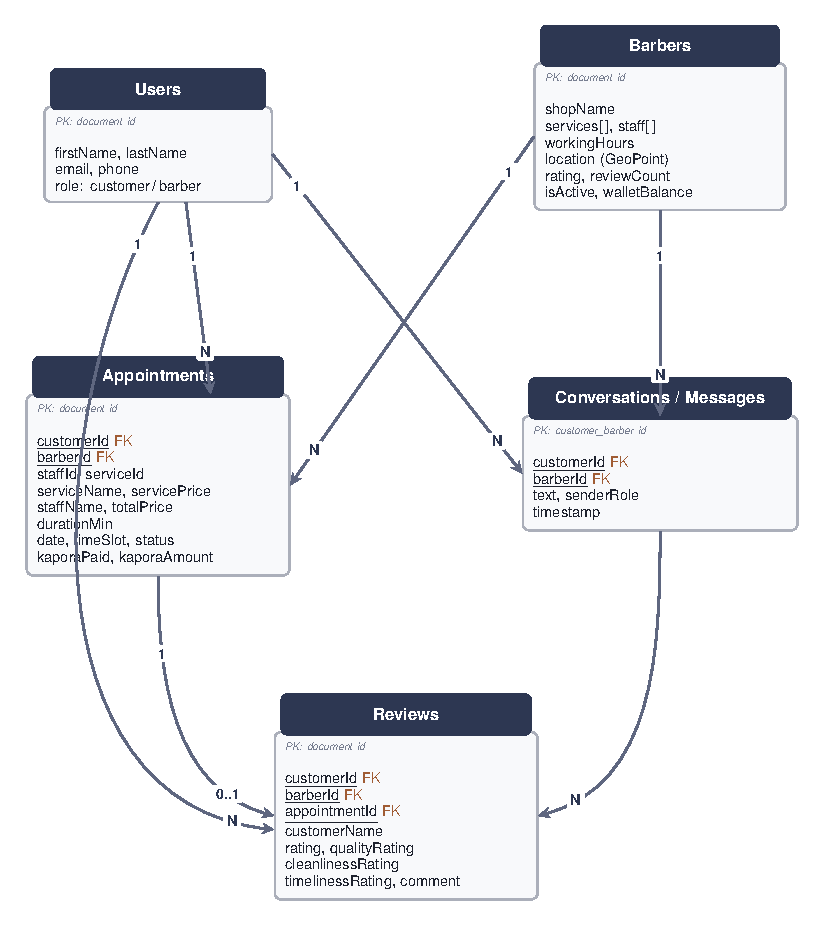
\includegraphics[width=0.82\textwidth]{erd}
  \caption{Entity-relationship diagram of the implemented Firestore data
  model. Underlined fields are reference (FK-style) fields; Firestore
  does not enforce them as true foreign keys. Cardinalities reflect the
  application logic (e.g. one appointment maps to at most one review,
  per the verified-only review rule).}
  \label{fig:erd}
\end{figure}

\begin{table}[t]
\caption{Firestore data model (as implemented).}
\label{tab:datamodel}
\centering
\footnotesize
\begin{tabular}{@{}p{0.20\columnwidth}p{0.70\columnwidth}@{}}
\toprule
\textbf{Collection} & \textbf{Key fields} \\
\midrule
\texttt{users} & firstName, lastName, email, phone, role
                 (customer\,/\,barber) \\
\texttt{barbers} & shopName, services[], staff[], workingHours,
                   location (GeoPoint), rating, reviewCount, isActive,
                   walletBalance \\
\texttt{appointments} & customerId, barberId, staffId, serviceId,
                       serviceName, servicePrice, staffName, totalPrice,
                       durationMin, date, timeSlot, status, kaporaPaid,
                       kaporaAmount \\
\texttt{reviews} & customerId, barberId, appointmentId, customerName,
                   rating, qualityRating, cleanlinessRating,
                   timelinessRating, comment \\
\texttt{conversations} / \texttt{messages} & deterministic
                 customer\_\_barber id; messages with text, senderRole,
                 timestamp \\
\bottomrule
\end{tabular}
\end{table}

\subsection{Stage 3 -- Frontend (Mobile UI)}
The client was implemented with React~Native instead of Kotlin. The
Customer side is complete end to end: a Home screen with a
\texttt{react-native-maps} map, search, a preferences sheet (sort by
recommended / nearest / top-rated / best-price, service-type chips,
open-now switch, and a draggable distance-radius slider), a shop-detail
screen, a slot-based booking screen, an appointments list with
upcoming/past/cancelled tabs and status badges, a messaging screen, a
rating screen, and a profile. The rating screen captures three separate
dimensions---service quality, cleanliness, and timeliness---in addition
to an overall score and a free-text comment, giving more actionable
feedback than a single star rating. The Barber side provides a four-step
registration wizard, a dashboard, an appointments view, and a shop
profile. Discovery distance is computed on the client with the Haversine
formula against the device's GPS position obtained via
\texttt{expo-location}.

\subsection{Stage 4 -- Backend Integration and Logic}
Authentication uses Firebase email/password; profiles and barber-shop
placeholders are created on sign-up. The booking flow writes an
appointment document, and double-booking is prevented by reading the
day's existing \texttt{pending}/\texttt{confirmed} slots and disabling
them in the UI, taking service duration into account. Appointment status
transitions (pending, confirmed, completed, cancelled) are persisted, and
cancellation is allowed only up to two hours before the slot.

The payment step is a deliberately scoped mock, but it is no longer a
bare field-completeness check. The implemented \texttt{PaymentScreen}
validates the card number with the Luhn check-digit
algorithm~\citep{luhn1960verifying} (\texttt{isValidLuhn} in
\texttt{src/utils/luhn.ts}), in addition to checking that the expiry,
CVV, and cardholder fields are filled; only a Luhn-valid number unlocks
the ``pay deposit'' action. The function was verified with a dedicated
test script against 6 known card numbers (industry-standard test
numbers such as \texttt{4242\,4242\,4242\,4242}, plus deliberately
corrupted variants) and against a generated 100-card set (50 valid, 50
invalid), achieving 100\% classification accuracy on both -- the exact
test specified in the proposal's Experimental Results plan. On a
successful charge the flow transfers a 10\% deposit (``kapora'') to the
barber's wallet balance and creates the appointment. No real payment
gateway is involved; this remains a simulated transaction by design.

\subsection{Stage 5 -- AI Module Research (Future Integration)}
No computer-vision code exists in the repository. The intended direction
is documented rather than built: a head-shape/face-region detector based
on the Viola--Jones cascade~\citep{viola2001rapid} (or a modern
equivalent) feeding a rule-based style recommender. This stage is
explicitly future work.

\subsection{Stage 6 -- Usability Testing and Quality Assurance}
The planned evaluation method is inspection- and questionnaire-based
usability assessment in the tradition of Nielsen's usability inspection
methods~\citep{nielsen1994usability}, with the System Usability Scale (SUS)
as the summative instrument. Aside from the Luhn unit test in
\texttt{src/utils/luhn.test.ts} (Section~\ref{sec:exp}), the repository
contains no automated UI tests, no continuous-integration configuration,
and no recorded usability-study data, so the outcomes of this stage are
reported as pending in Section~\ref{sec:exp}.

%-----------------------------------------------------------------------
\section{Experimental Results}
\label{sec:exp}
%-----------------------------------------------------------------------
To respect academic integrity, this section separates what has been
\emph{verified} from what is only \emph{planned}. At the time of writing
the repository contains no automated UI test suite, CI pipeline, or
survey data, so usability and runtime-performance numbers cannot be
reported yet. One quantitative result does exist -- the Luhn payment
check has been unit-tested and is reported with real numbers below. The
measurement plan for the remaining targets specifies how each will be
evaluated, with concrete TODOs for the missing numbers.

\subsection{Functional verification (evidenced)}
The following behaviours are verifiable from the implemented code and a
running build:
\begin{itemize}
  \item Discovery filters and sorts (nearest, top-rated, best-price,
        open-now, distance radius) operate over both seeded Firestore
        data and a built-in mock fallback.
  \item Booking disables already-taken slots for the selected day and
        barber, preventing double-booking in the UI.
  \item The verified-review rule holds: a ``Rate'' action appears only on
        \texttt{completed} appointments, and a second review for the same
        appointment is blocked.
  \item Messaging updates in real time via Firestore
        \texttt{onSnapshot} subscriptions.
  \item \textbf{Payment validation (Luhn).} \texttt{isValidLuhn} was
        tested against 6 known card numbers (industry-standard test
        numbers and deliberately corrupted variants) and against a
        generated 100-card set (50 valid, 50 invalid), via
        \texttt{src/utils/luhn.test.ts}. Result: 6/6 known-card checks
        passed and 100/100 (100\%) classification accuracy on the
        generated set -- the exact test specified in the proposal.
\end{itemize}

\subsection{Usability and HCI metrics (planned)}
\begin{itemize}
  \item \textbf{System Usability Scale (SUS).} Target $\geq 75$ (``high
        usability''). Method: standard 10-item SUS administered after a
        guided task set.
        % TODO(team): run SUS with N>=5 participants and paste the mean
        % SUS score and per-item results here.
  \item \textbf{Task-completion rate.} Percentage of users who complete a
        booking without assistance or error.
        % TODO(team): record completion/error counts and report.
  \item \textbf{Booking efficiency.} Average in-app booking time vs.\ a
        phone/walk-in baseline.
        % TODO(team): time the task and report mean +/- SD.
\end{itemize}

\subsection{Remaining technical validation (planned)}
\begin{itemize}
  \item \textbf{Discovery latency.} The proposal's ``$<$200\,ms
        geospatial query'' target should be reframed for the actual
        architecture: distance is computed on the client and shop data is
        fetched with a single-filter Firestore query. The meaningful
        metric is barber-list load time (network fetch + client sort).
        % TODO(team): measure cold/warm load time over the seeded data
        % set and report median/95th percentile.
  \item \textbf{Booking integrity.} Concurrency behaviour under
        simultaneous bookings of the same slot.
        % TODO(team): the current guard is client-side only; add a
        % Firestore transaction/security rule and test concurrent writes.
\end{itemize}

%-----------------------------------------------------------------------
\section{Conclusions and Future Works}
\label{sec:concl}
%-----------------------------------------------------------------------
\textbf{Discovery} is delivered: GPS, map, and client-side distance
ranking with practical filters work over real seeded shops near IZTECH.
\textbf{Interaction} is delivered end to end for customers (booking,
cancellation, real-time messaging, rating) and substantially for barbers
(registration wizard, dashboard, appointment management).
\textbf{Reliability} is substantially delivered: the verified-only
review rule is enforced, and the deposit step is secured by a
unit-tested Luhn check (100\% accuracy on a 100-card set), though it
remains a simulated transaction with no real payment gateway by design.
The largest deviation from the proposal is the stack
itself---Expo/React~Native and Firebase replaced Kotlin, .NET, and
PostgreSQL---which let a small team ship a cross-platform, end-to-end
prototype quickly at the cost of a custom server and some originally
promised server-side guarantees.

Even at prototype scale the work has value. It demonstrates a concrete,
testable mechanism for the recurring trust problem in service-review
platforms (binding feedback to a completed transaction), and it packages
location discovery, slot-based booking, and direct messaging into one
coherent HCI flow grounded in established usability
principles~\citep{shneiderman2016designing}.

\textbf{Future works}, in priority order: (1) move the double-booking
guard into a Firestore transaction/security rule; (2) run the SUS-based
usability evaluation~\citep{nielsen1994usability} and the performance
measurements specified in Section~\ref{sec:exp}; (3) finalise remaining
barber-side polish and add automated tests and CI; and (4) build the AI
head-shape styling module~\citep{viola2001rapid}, the proposal's
explicitly forward-looking feature.

%-----------------------------------------------------------------------
\section{Weekly Schedule / Project Plan}
%-----------------------------------------------------------------------
Table~\ref{tab:gantt} recolours the proposal's 12-week plan to reflect
the real state of the repository:
\colorbox{doneG}{\strut finished},
\colorbox{progB}{\strut in progress}, and
\colorbox{planY}{\strut planned / future}. Task labels are updated where
the implementation diverged from the plan (e.g.\ React~Native instead of
Kotlin, Firebase instead of .NET/PostgreSQL). Note that the actual coding
activity was concentrated in a short, intense sprint rather than spread
evenly across twelve calendar weeks; the columns therefore represent
plan phases, while the colours represent delivery status as of this
report.

\begin{table}[h!]
\caption{Project plan, recoloured by actual delivery status.
         Green = finished, blue = in progress, yellow = planned/future.}
\label{tab:gantt}
\centering
\footnotesize
\setlength{\tabcolsep}{3pt}
\renewcommand{\arraystretch}{1.3}
\resizebox{\textwidth}{!}{%
\begin{tabular}{|p{0.30\textwidth}|c|c|c|c|c|c|c|c|c|c|c|c|}
\hline
\textbf{Task} & \textbf{W1} & \textbf{W2} & \textbf{W3} & \textbf{W4}
 & \textbf{W5} & \textbf{W6} & \textbf{W7} & \textbf{W8} & \textbf{W9}
 & \textbf{W10} & \textbf{W11} & \textbf{W12} \\
\hline
Requirement analysis \& personas
 & \cD & \cD &     &     &     &     &     &     &     &     &     &     \\
\hline
UI/UX wireframing (low-fi)
 &     & \cD & \cD &     &     &     &     &     &     &     &     &     \\
\hline
Data modeling (Firestore) \& ERD
 &     &     & \cD & \cD &     &     &     &     &     &     &     &     \\
\hline
Backend / data layer (Firebase; was .NET)
 &     &     &     & \cD & \cD & \cD & \cD &     &     &     &     &     \\
\hline
Mobile UI (React Native; was Kotlin)
 &     &     &     &     & \cD & \cD & \cD & \cD &     &     &     &     \\
\hline
Real-time messaging
 &     &     &     &     &     &     & \cD & \cD & \cD &     &     &     \\
\hline
Payment (mock deposit, Luhn-secured)
 &     &     &     &     &     &     & \cD & \cD & \cD &     &     &     \\
\hline
AI infrastructure research (head-shape)
 &     &     &     &     &     &     &     & \cY & \cY & \cY &     &     \\
\hline
System integration \& debugging
 &     &     &     &     &     &     &     &     & \cD & \cD & \cD &     \\
\hline
Usability testing (SUS) \& final fixes
 &     &     &     &     &     &     &     &     &     &     & \cY & \cY \\
\hline
Final demo \& presentation
 &     &     &     &     &     &     &     &     &     &     &     & \cY \\
\hline
\end{tabular}%
}
\end{table}

%-----------------------------------------------------------------------
\bibliographystyle{chicago}
\bibliography{literature}

\end{document}
